\chapter{BLI Modeling Phase}

\section{Baseline Design}
\subsection{Baseline Thrust Requirements}
\section{BLI Modeling}
\subsection{Airframe Model}
\subsection{Power Balance and Drag Book-keeping}
\subsection{Inlet Model}
\subsection{PC Model}
\subsubsection{General Model Architecture and Algorithm}

\section{Experiment 1 Results}

\subsection{Flight Condition Variation}

\subsubsection{Angle of Attack Impact}
	%%
	\begin{figure}[p]
	\centering
	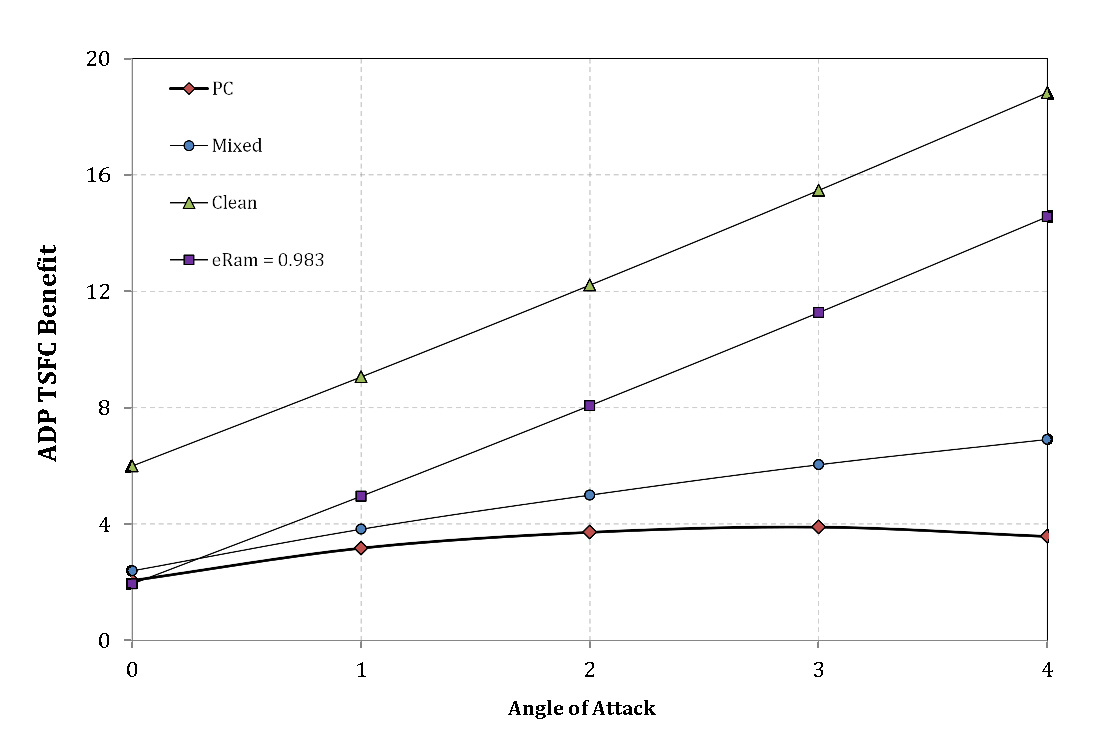
\includegraphics[width=0.8\textwidth]{alpha_sweeps.eps}
	\caption{Angle of attack performance variation for different fidelity models.}
	\label{alpha_sweeps}
	\end{figure}
	%%

\subsection{Design Space Variation}

\subsection{Influence of Inlet Aperture Shape}

\subsection{Influence of Engine Number}

\subsection{Mass Flow Variation}

\subsection{Influence of the pre-entry zone}

\section{Stall Margin Test Experimental Setup}

\subsection{Stall Margin Criteria and Allowables}

\section{Experiment 2 Results}

\subsection{Determining Design Stall Margin and Efficiency Trade-off}

\section{Summary of BLI Modeling Phase}